\section{Budgeted Actor Refinement}
\label{sec:method}

Let $\D$ contain transitions $(s,a,r,s')$ and let $\widehat Q$ denote the first online critic. BAR maintains actors $\mu_{1:K}$ with separate parameters and Adam states. At a delayed actor update, the critic is held fixed while the actors are updated in order on the same minibatch. Define $h=T/K$.

\paragraph{Exact implementation-level references and scales.}
The proximal and linearized paths use different first-hop scale locations. For BAR-Prox, the first and later references are
\begin{align}
 r^{\rm P}_1&=a, & z^{\rm P}_1&=\mu^{\rm pre}_1(s),\label{eq:prox_refs_a}\\
 r^{\rm P}_k&=\sg\mu^{\rm post}_{k-1}(s), & z^{\rm P}_k&=r^{\rm P}_k,\quad k\ge2.\label{eq:prox_refs_b}
\end{align}
where ``pre'' and ``post'' refer to the current actor before its update and the predecessor after its update. For BAR-Lin,
\begin{align}
 r^{\rm L}_1&=z^{\rm L}_1=a,\label{eq:lin_refs_a}\\
 r^{\rm L}_k&=z^{\rm L}_k=\sg\mu^{\rm post}_{k-1}(s),\quad k\ge2.\label{eq:lin_refs_b}
\end{align}
For path $X\in\{\rm P,L\}$,
\begin{equation}
 C^X_k=\sg\!\left(\E_s|\widehat Q(s,z^X_k)|+\epsilon\right).
\label{eq:qscale}
\end{equation}
Thus later hops use the reference action in both paths, but the first proximal hop uses the current actor output while the first linearized hop uses the dataset action. We therefore call BAR-Lin an action-metric-matched linearized control, not an exactly scale-identical first-hop integrator.

The proximal-loss actor update is one Adam step on
\begin{equation}
\begin{split}
 \mathcal L^{\rm P}_{k}(\theta_k)
 ={}&-\frac{2h}{C^{\rm P}_k}\E_s\widehat Q(s,\mu_{\theta_k}(s))\\
 &+\E_s\frac{\|\mu_{\theta_k}(s)-r^{\rm P}_k(s)\|_2^2}{d}.
\end{split}
\label{eq:prox_loss}
\end{equation}
The linearized path constructs
\begin{equation}
 a_k^{\rm tar}=\Pi_{\A}\!\left[r^{\rm L}_k
 +\frac{dh}{C^{\rm L}_k}\nabla_a\widehat Q(s,a)\big|_{a=r^{\rm L}_k}\right]
\label{eq:lin_target}
\end{equation}
and performs one MSE update toward $a_k^{\rm tar}$. The factor $d$ matches the action-coordinate-averaged quadratic cost. Projection and neural regression make this a projected target-fitting control, not an exact Euler trajectory.

After actor 1 is updated, its Polyak target and the target critic are updated. The critic subsequently bootstraps through the target copy $\mu_1^-$ with TD3 target smoothing, while evaluation uses $\mu_K$. Figure~\ref{fig:architecture} summarizes the route.

\begin{figure}[t]
\centering
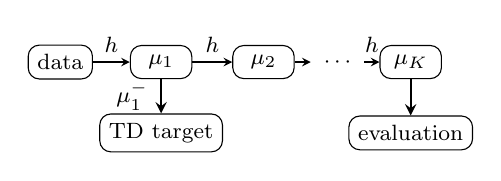
\begin{tikzpicture}[x=1cm,y=1cm,>=stealth,every node/.style={font=\footnotesize}]
  \node[draw,rounded corners,minimum width=.72cm,minimum height=.42cm] (d) at (0,0) {data};
  \node[draw,rounded corners,minimum width=.78cm,minimum height=.42cm] (p1) at (1.28,0) {$\mu_1$};
  \node[draw,rounded corners,minimum width=.78cm,minimum height=.42cm] (p2) at (2.58,0) {$\mu_2$};
  \node at (3.52,0) {$\cdots$};
  \node[draw,rounded corners,minimum width=.78cm,minimum height=.42cm] (pk) at (4.45,0) {$\mu_K$};
  \draw[->] (d)--node[above] {$h$}(p1);
  \draw[->] (p1)--node[above] {$h$}(p2);
  \draw[->] (p2)--(3.18,0);
  \draw[->] (3.86,0)--node[above] {$h$}(pk);
  \node[draw,rounded corners,minimum width=1.18cm,minimum height=.42cm] (td) at (1.28,-.9) {TD target};
  \node[draw,rounded corners,minimum width=1.18cm,minimum height=.42cm] (ev) at (4.45,-.9) {evaluation};
  \draw[->,thick] (p1)--node[left,xshift=-1pt] {$\mu_1^-$}(td);
  \draw[->,thick] (pk)--(ev);
\end{tikzpicture}
\caption{BAR actor dataflow. The first actor's target copy supplies Bellman target actions; the persistent final actor is evaluated.}
\label{fig:architecture}
\end{figure}

\paragraph{Complexity and estimand.}
Relative to one actor, actor-update time and actor parameter/optimizer memory scale as $O(K)$; critic updates, replay samples, and the number of critic steps are unchanged. The complete sweep is not actor-compute matched. Accordingly, $K$ indexes the implemented bundle: local coefficient $T/K$, refinement depth, persistent actor capacity, re-centering, normalization path, routing, and actor compute all change together.
